\chapter{Covariant elektromagnetisme}\label{ch:b3:covariant-electromagnetism}

Een koperdraad voert tien ampère. Zijn elektronen driften met een tiende
millimeter per seconde --- trager dan een slak --- en de draad is tot in
fantastische precisie elektrisch neutraal. Toch voelt een lading die
ernaast meebeweegt een meetbare trek. Bekeken vanuit het eigen stelsel van
die lading verdampt de ``magnetische'' verklaring: de lading is in rust,
en een rustende lading voelt in het geheel geen magnetische kracht. Wat
haar in dat stelsel trekt is een \emph{elektrisch} veld --- opgeroepen
door de relativiteitstheorie zelf, want de \omterm{prop:b3:relativistic-kinematics:contraction}{lengtekrimp} brengt de twee
ladingsstromen in de draad met één deel op $10^{24}$ uit balans.
Magnetisme is elektriciteit gezien vanaf een bewegende stoel. Dit
hoofdstuk herschrijft het elektromagnetisme van het volume van jaar 2 in
de taal van de vorige drie hoofdstukken: \omterm{def:b3:covariant-electromagnetism:fourvector}{viervectoren} voor lading en
potentiaal, één antisymmetrische tensor die $\vect E$ en $\vect B$
samenhoudt, en de vier vergelijkingen van Maxwell die inklappen tot twee
regels die in elk \omterm{thm:b3:relativistic-kinematics:postulates}{inertiaalstelsel} hetzelfde luiden. Behalve elegantie
levert dat werkende natuurkunde op: hoe velden transformeren, waarom het
veld van een snelle lading tot een pannenkoek platslaat, en waarom het
licht van een relativistisch elektron als een koplamp naar voren zwenkt
--- het beginsel van de synchrotronlichtbronnen die vandaag eiwitten en
batterijen doorlichten.

\section{Viervectoren voor lading en stroom}

\begin{definition}[Viervectoren]\label{def:b3:covariant-electromagnetism:fourvector}
\index{viervector}
Een \emph{viervector} is een viertal $a^\mu = (a^0, \vect a)$, $\mu =
0, 1, 2, 3$, waarvan de componenten onder een boost precies zo mengen als
$(ct,
\vect r)$:
\[
a'^0 = \gamma(a^0 - \beta a^1) , \qquad
a'^1 = \gamma(a^1 - \beta a^0) , \qquad
a'^{2,3} = a^{2,3}
\]
voor een boost met $\beta c$ langs $x$. Elk tweetal viervectoren geeft
het invariante scalair product $a\cdot b = a^0b^0 - \vect a\cdot\vect b$,
in elk stelsel hetzelfde getal --- het patroon achter $c^2t^2 - x^2$ en
$E^2 - p^2c^2$. De positie $(ct, \vect r)$ en de \omterm{def:b3:relativistic-dynamics:four-momentum}{viererimpuls}
$(E/c, \vect p)$ hebben we al; het elektromagnetisme levert er nu drie
bij: stroom, potentiaal en golfvector.
\end{definition}

\begin{proposition}[De vierstroom en het ladingsbehoud]\label{prop:b3:covariant-electromagnetism:fourcurrent}
\index{vierstroom}
De ladingsdichtheid $\rho$ en de stroomdichtheid $\vect\jmath$ vormen de
vierstroom
\[
J^\mu = (\rho c,\ \vect\jmath\,) :
\]
een ladingswolk met eigen dichtheid $\rho_0$ die met $\vect u$ beweegt
heeft $J^\mu = \rho_0\gamma_u(c, \vect u)$ --- de dichtheid groeit met
$\gamma_u$ omdat het volume van de wolk krimpt, terwijl de lading zelf
invariant is (een beslissend experimenteel feit: atomen met snelle
binnenelektronen blijven exact neutraal). Het ladingsbehoud is de
invariante uitspraak
\[
\frac{\partial(\rho c)}{\partial(ct)} +
\operatorname{div}\vect\jmath = 0 ,
\]
de continuïteitsvergelijking van het volume van jaar 2, nu zichtbaar
dezelfde wet voor alle waarnemers.
\end{proposition}

\begin{proof}[Gedeeltelijk bewijs]
De bewegende wolk: een doos met eigen volume $V_0$ bevat de lading
$\rho_0
V_0$; in het lab is de doos tot $V_0/\gamma_u$ gekrompen, dus
$\rho =
\gamma_u\rho_0$, en $\vect\jmath = \rho\vect u$ volgens de
definitie van een stroomdichtheid. Dat $(\rho c, \vect\jmath)$ dan als
een \omterm{def:b3:covariant-electromagnetism:fourvector}{viervector} transformeert volgt omdat het gelijk is aan $\rho_0/c$
maal de viersnelheid $\gamma_u(c, \vect u)$, die per constructie zelf een
\omterm{def:b3:covariant-electromagnetism:fourvector}{viervector} is. De invariantie van de lading is een experimenteel gegeven.
\end{proof}

\section{Eén tensor voor beide velden}

\begin{definition}[Vierpotentiaal en veldtensor]\label{def:b3:covariant-electromagnetism:tensor}
\index{vierpotentiaal}\index{veldtensor}
De potentialen van het volume van jaar 2 voegen zich samen tot de
vierpotentiaal
\[
A^\mu = \Big(\frac{V}{c},\ \vect A\Big) ,
\]
en de meetbare velden $\vect E = -\vect\nabla V -
\partial_t\vect A$ en
$\vect B = \operatorname{\vect{curl}}\vect A$ zijn de zes onafhankelijke
componenten van één antisymmetrisch schema, de
\emph{elektromagnetische veldtensor}
\[
F^{\mu\nu} =
\begin{pmatrix}
0 & -E_x/c & -E_y/c & -E_z/c\\
E_x/c & 0 & -B_z & B_y\\
E_y/c & B_z & 0 & -B_x\\
E_z/c & -B_y & B_x & 0
\end{pmatrix} .
\]
$\vect E$ en $\vect B$ zijn geen twee velden maar zes gezichten van één
voorwerp; welk gezicht een waarnemer ``elektrisch'' noemt, hangt van zijn
beweging af.
\end{definition}

\begin{theorem}[Maxwell, covariant]\label{thm:b3:covariant-electromagnetism:maxwell}
\index{vergelijkingen van Maxwell!covariante vorm}
De vier vergelijkingen van Maxwell uit het volume van jaar 2 zijn de
componentvorm van twee stelselonafhankelijke uitspraken: het paar met
bronnen (Gauss en Ampère--Maxwell) luidt
\[
\sum_\mu \partial_\mu F^{\mu\nu} = \mu_0\,J^\nu ,
\]
en het bronloze paar (geen monopolen, Faraday) is de identiteit die
waarborgt dat $F$ uit een \omterm{def:b3:covariant-electromagnetism:tensor}{vierpotentiaal} volgt. De lorentzkracht is
$\dd p^\mu/\dd\tau = qF^{\mu\nu}u_\nu$ --- de krachtwet, magnetisme
inbegrepen, in één regel. Omdat beide leden van elke vergelijking op
dezelfde manier transformeren, \emph{heeft de theorie van Maxwell geen
enkele correctie nodig om relativistisch te zijn}: zij was het eerste
voltooide stuk van de relativiteitstheorie, geboren in 1865.
\end{theorem}

\begin{proof}[Gedeeltelijk bewijs]
Werk de component $\nu = 0$ uit: $\sum_i\partial_i(E_i/c) =
\mu_0\rho c$,
dat wil zeggen $\operatorname{div}\vect E = \rho/\varepsilon_0$ (met $c^2 = 1/\mu_0\varepsilon_0$). De component $\nu = 1$ verzamelt
$-\partial_t(E_x/c^2) + (\partial_yB_z - \partial_zB_y)
= \mu_0 j_x$: de
$x$-component van Ampère--Maxwell. De overige componenten herhalen het
patroon; het bronloze paar is de gelijkheid van gekruiste tweede
afgeleiden van $A^\mu$ (nagegaan in
\cref{exo:b3:covariant-electromagnetism:3}). Dat $F^{\mu\nu}$ als een
tensor met twee indices transformeert --- elke index als een \omterm{def:b3:covariant-electromagnetism:fourvector}{viervector}
--- wordt aangenomen; de gevolgen ervan zijn de volgende propositie.
\end{proof}

\section{Hoe de velden transformeren}

\begin{proposition}[Transformatie van de velden]\label{prop:b3:covariant-electromagnetism:transform}
\index{transformatie van de velden}
Voor een boost met snelheid $\vect v = v\,\vect e_x$: de componenten
\emph{langs} de beweging blijven onaangeroerd, de dwarse mengen,
\[
E'_x = E_x , \qquad
E'_y = \gamma(E_y - vB_z) , \qquad
E'_z = \gamma(E_z + vB_y) ,
\]
\[
B'_x = B_x , \qquad
B'_y = \gamma\Big(B_y + \frac{v}{c^2}E_z\Big) , \qquad
B'_z = \gamma\Big(B_z - \frac{v}{c^2}E_y\Big) .
\]
Kort samengevat, dwars op de boost: $\vect E' = \gamma(\vect E +
\vect v\wedge\vect B)_\perp$ en $\vect B' = \gamma(\vect B - \vect
v\wedge\vect E/c^2)_\perp$. Een zuivere $\vect B$ in het ene stelsel is $\vect
E$ én
$\vect B$ in een ander: de velden zijn één verschijnsel.
\end{proposition}
\admitted

\begin{example}[Magnetisme uit een neutrale draad]\label{ex:b3:covariant-electromagnetism:wire}
Een neutrale draad voert stroom: het positieve rooster in rust, de
elektronen driftend. Boost voor een proeflading die ernaast meebeweegt
naar haar stelsel: de twee ladingsstromen krimpen \emph{verschillend} (zij
hebben verschillende snelheden), de draad krijgt de netto lijnlading
$\lambda' =
-\gamma vI/c^2$, en haar radiale elektrische veld trekt aan de
lading met precies de kracht die het lab $q\vect v\wedge\vect B$ noemde.
Magnetisme is hoe de tweede-ordeterm $v u/c^2$ van de
relativiteitstheorie eruitziet wanneer $10^{28}$ elementaire ladingen per
meter samenspannen: elk effect is fantastisch klein, maar de draad is tot
in nog grotere precisie neutraal, zodat het minieme onevenwicht het hele
verhaal is (\cref{pb:b3:covariant-electromagnetism:1}).
\end{example}

\begin{omfigure}
\begin{tikzpicture}[font=\small, >=Stealth]
  % lab frame
  \begin{scope}
    \draw[thick, fill=omExo!10] (-0.2,0) rectangle (5.4,0.75);
    \foreach \x in {0.3,1.3,2.3,3.3,4.3} \node[omThm] at (\x,0.52) {$\oplus$};
    \foreach \x in {0.8,1.8,2.8,3.8,4.8} {\node[omDef] at (\x,0.22) {$\ominus$};
      \draw[->, omDef] (\x+0.16,0.22) -- (\x+0.42,0.22);}
    \fill[omProp] (2.6,-1.15) circle (2.6pt);
    \draw[->, omProp, thick] (2.75,-1.15) -- (3.55,-1.15);
    \node[anchor=west] at (3.65,-1.15) {$q$, snelheid $v$};
    \draw[->, very thick] (2.6,-0.95) -- (2.6,-0.35);
    \node[anchor=west, font=\footnotesize] at (2.7,-0.62) {$q\vect v\wedge\vect B$};
    \node at (2.6,1.35) {lab: draad neutraal, kracht magnetisch};
  \end{scope}
  % charge frame
  \begin{scope}[xshift=7.8cm]
    \draw[thick, fill=omExo!10] (-0.2,0) rectangle (5.4,0.75);
    \foreach \x in {0.25,1.15,2.05,2.95,3.85,4.75} {\node[omThm] at (\x,0.52) {$\oplus$};
      \draw[->, omThm] (\x-0.14,0.72) -- (\x-0.4,0.72);}
    \foreach \x in {0.7,1.9,3.1,4.3} \node[omDef] at (\x,0.22) {$\ominus$};
    \fill[omProp] (2.6,-1.15) circle (2.6pt);
    \node[anchor=west] at (2.75,-1.35) {$q$ in rust};
    \draw[->, very thick] (2.6,-0.95) -- (2.6,-0.35);
    \node[anchor=west, font=\footnotesize] at (2.7,-0.62) {$q\vect E'$};
    \node at (2.6,1.35) {stelsel van de lading: draad geladen, kracht elektrisch};
  \end{scope}
\end{tikzpicture}

{\small Eén kracht, twee boekhoudingen. Lab: de stroom in de neutrale
draad maakt $\vect B$, en de bewegende lading voelt $q\vect v\wedge\vect B$. Stelsel van de lading: het positieve rooster beweegt nu en krimpt, de
elektronen (daar trager) spreiden uit; de draad is netto geladen en zijn
$\vect E'$ doet het trekwerk. Zelfde proef, zelfde uitkomst.}
\end{omfigure}

\begin{example}[Het platgeslagen veld van een snelle lading]\label{ex:b3:covariant-electromagnetism:pancake}
Transformeer het coulombveld van een lading naar het stelsel waarin zij
met $\gamma \gg 1$ beweegt: het veld in de lengterichting blijft
ongewijzigd terwijl het dwarse met $\gamma$ wordt vermenigvuldigd. Het
ooit bolvormige veld plat af tot een schijf met openingshoek $\sim 1/\gamma$ rond het vlak door de lading --- vergezeld, dwars op de
beweging, door een magnetische ring $B' = vE'/c^2$. Voor een stilstaande
waarnemer is de passage van een LHC-proton ($\gamma \approx 7000$) een
klap van minder dan een picoseconde van vrijwel gekruiste $\vect E$ en
$\vect B$: bijna een lichtpuls --- de reden dat snelle bundels met
materie praten zoals fotonen dat doen.
\end{example}

\begin{omfigure}
\begin{tikzpicture}[font=\small, >=Stealth]
  % static charge
  \begin{scope}
    \fill[omThm] (0,0) circle (2.6pt);
    \foreach \a in {0,30,...,330} \draw[->, omDef] (\a:0.25) -- (\a:1.75);
    \node at (0,-2.5) {in rust: isotroop coulombveld};
  \end{scope}
  % moving charge
  \begin{scope}[xshift=8.0cm]
    \fill[omThm] (0,0) circle (2.6pt);
    \draw[->, very thick] (0.3,-2.1) -- (1.5,-2.1) node[right] {$v \approx c$};
    \foreach \a/\l in {90/1.95, 75/1.5, 105/1.5, 60/0.85, 120/0.85,
                       270/1.95, 255/1.5, 285/1.5, 240/0.85, 300/0.85,
                       0/0.35, 180/0.35, 30/0.45, 150/0.45, 210/0.45, 330/0.45}
      \draw[->, omDef] (\a:0.25) -- (\a:\l);
    \node at (0,-2.5) {};
    \node at (0.3,-2.65) {};
    \node at (0,-2.9) {};
  \end{scope}
  \node at (8.0,-2.5) {bewegend: veld platgeslagen tot $\sim 1/\gamma$};
\end{tikzpicture}

{\small Het elektrische veld van een puntlading, in rust en bij hoge
snelheid: boosten vermenigvuldigt de dwarse componenten met $\gamma$ en
laat de componenten in de lengterichting met rust, waardoor het veld tot
een schijf loodrecht op de beweging wordt geperst.}
\end{omfigure}

\section{Invarianten, licht en het koplampeffect}

\begin{proposition}[De twee veldinvarianten]\label{prop:b3:covariant-electromagnetism:invariants}
\index{veldinvarianten}
Uit $F^{\mu\nu}$ zijn precies twee onafhankelijke scalairen te bouwen:
\[
E^2 - c^2B^2
\qquad\text{en}\qquad
\vect E\cdot\vect B ,
\]
in elk \omterm{thm:b3:relativistic-kinematics:postulates}{inertiaalstelsel} dezelfde. Gevolgen: is ergens $E > cB$ (met
$\vect E\cdot\vect B = 0$), dan ziet een of ander stelsel daar een zuiver
elektrisch veld; is $E < cB$, dan ziet een of ander stelsel een zuiver
magnetisch veld; en een vlakke lichtgolf, met $E = cB$ en $\vect E\perp\vect B$, heeft \emph{beide} invarianten nul --- zij is licht in elk
stelsel: geen enkele boost maakt er een statisch veld van, alleen een
roodverschuiving. Men kan een lichtgolf niet inhalen; de vraag die
Einstein zich als jongen stelde beantwoordt zichzelf in twee invarianten.
\end{proposition}

\begin{proof}[Gedeeltelijk bewijs]
Ga de invariantie onder de standaardboost na door
\cref{prop:b3:covariant-electromagnetism:transform} rechtstreeks in te
vullen (\cref{exo:b3:covariant-electromagnetism:6}); dat er geen derde
onafhankelijke invariant bestaat wordt aangenomen. Voor de golf: uit $E = cB$ en de loodrechtheid volgt dat beide nul zijn; een stelsel met een
statisch veld zou een invariant ongelijk nul nodig hebben.
\end{proof}

\begin{proposition}[Viergolfvector, doppler en aberratie]\label{prop:b3:covariant-electromagnetism:wavevector}
\index{aberratie}\index{koplampeffect}
De frequentie en de richting van een vlakke golf vormen de nulviervector
$k^\mu = (\omega/c, \vect k)$, $\|\vect k\| = \omega/c$. Hem
transformeren geeft in één klap de relativistische dopplerformule van
\cref{ch:b3:relativistic-kinematics} en de \emph{aberratie} van
richtingen:
\[
\cos\theta' = \frac{\cos\theta - \beta}{1 - \beta\cos\theta} .
\]
Achterstevoren gelezen: een bron die in haar ruststelsel isotroop straalt
bundelt in het lab de helft van haar licht in de voorwaartse kegel $\theta
\lesssim 1/\gamma$: het \emph{\omterm{prop:b3:covariant-electromagnetism:wavevector}{koplampeffect}}. Een elektron dat met $\gamma \sim 10^4$ in een opslagring rondgaat zwenkt een zoeklicht van
röntgenstraling van $\qty{0.1}{mrad}$ rond de ring --- het
synchrotronlicht dat de bundellijnen voor eiwitkristallografie vult.
\end{proposition}

\begin{proof}[Gedeeltelijk bewijs]
De fase $\omega t - \vect k\cdot\vect r = k^\mu x_\mu$ telt de golftoppen
die gebeurtenissen passeren --- een invariant --- dus moet $k^\mu$ als een
\omterm{def:b3:covariant-electromagnetism:fourvector}{viervector} transformeren. Pas de boost toe op $(\omega/c, k\cos\theta,
k\sin\theta, 0)$: de tijdcomponent geeft doppler, de verhouding van de
ruimtelijke componenten de aberratieformule. Stel $\theta' =
90^\circ$
(de zijwaartse straal in het stelsel van de bron): $\cos\theta =
\beta$,
dus $\theta \approx 1/\gamma$ voor $\gamma \gg 1$ --- de helft van de bol
vouwt in de voorwaartse kegel.
\end{proof}

\begin{omfigure}
\begin{tikzpicture}[font=\small, >=Stealth]
  % isotropic source
  \begin{scope}
    \fill[omThm] (0,0) circle (2.4pt);
    \foreach \a in {0,45,...,315} \draw[->, omExo] (\a:0.3) -- (\a:1.5);
    \node at (0,-2.2) {ruststelsel: isotroop};
  \end{scope}
  % beamed
  \begin{scope}[xshift=7.6cm]
    \fill[omThm] (0,0) circle (2.4pt);
    \draw[->, thick] (-1.9,0) -- (-0.6,0);
    \node at (-2.35,0) {$v$};
    \draw[->, omExo] (0.3,0.06) -- (2.6,0.55);
    \draw[->, omExo] (0.3,-0.06) -- (2.6,-0.55);
    \draw[->, omExo, very thick] (0.3,0) -- (2.9,0);
    \draw[->, omExo] (0.25,0.16) -- (1.5,1.0);
    \draw[->, omExo] (0.25,-0.16) -- (1.5,-1.0);
    \draw[->, omExo] (-0.1,0.28) -- (-0.5,1.0);
    \draw[->, omExo] (-0.1,-0.28) -- (-0.5,-1.0);
    \draw[dashed] (0,0) -- (3.1,0.85);
    \draw[dashed] (0,0) -- (3.1,-0.85);
    \node[anchor=west, font=\footnotesize] at (3.0,0.5) {$\sim 1/\gamma$};
    \node at (0.9,-2.2) {lab: een koplamp naar voren};
  \end{scope}
\end{tikzpicture}

{\small De aberratie vouwt de straling van een snelle bron in een
voorwaartse kegel met halve openingshoek $\sim 1/\gamma$: het
\omterm{prop:b3:covariant-electromagnetism:wavevector}{koplampeffect}, en het werkingsbeginsel van synchrotronlichtbronnen.}
\end{omfigure}

\begin{method}[Covariant werken]\label{met:b3:covariant-electromagnetism:method}
(1) Benoem de \omterm{def:b3:covariant-electromagnetism:fourvector}{viervectoren} die meespelen ($x^\mu$, $P^\mu$, $J^\mu$,
$A^\mu$, $k^\mu$) en geef de voorkeur aan hun invariante producten boven
componenten. (2) Splits om velden te transformeren in componenten langs en
dwars op de boost en pas
\cref{prop:b3:covariant-electromagnetism:transform} toe. (3) Toets de twee
invarianten voor en na --- de snelste foutendetector van het vak. (4)
Lijkt een magnetisch vraagstuk raadselachtig, rijd dan met de lading mee:
in haar stelsel werkt alleen $\vect E'$. (5) Vertrouw Maxwell: de
vergelijkingen hebben nooit relativistische ``correcties'' nodig, alleen
een relativistische lezing.
\end{method}

\begin{omfigure}
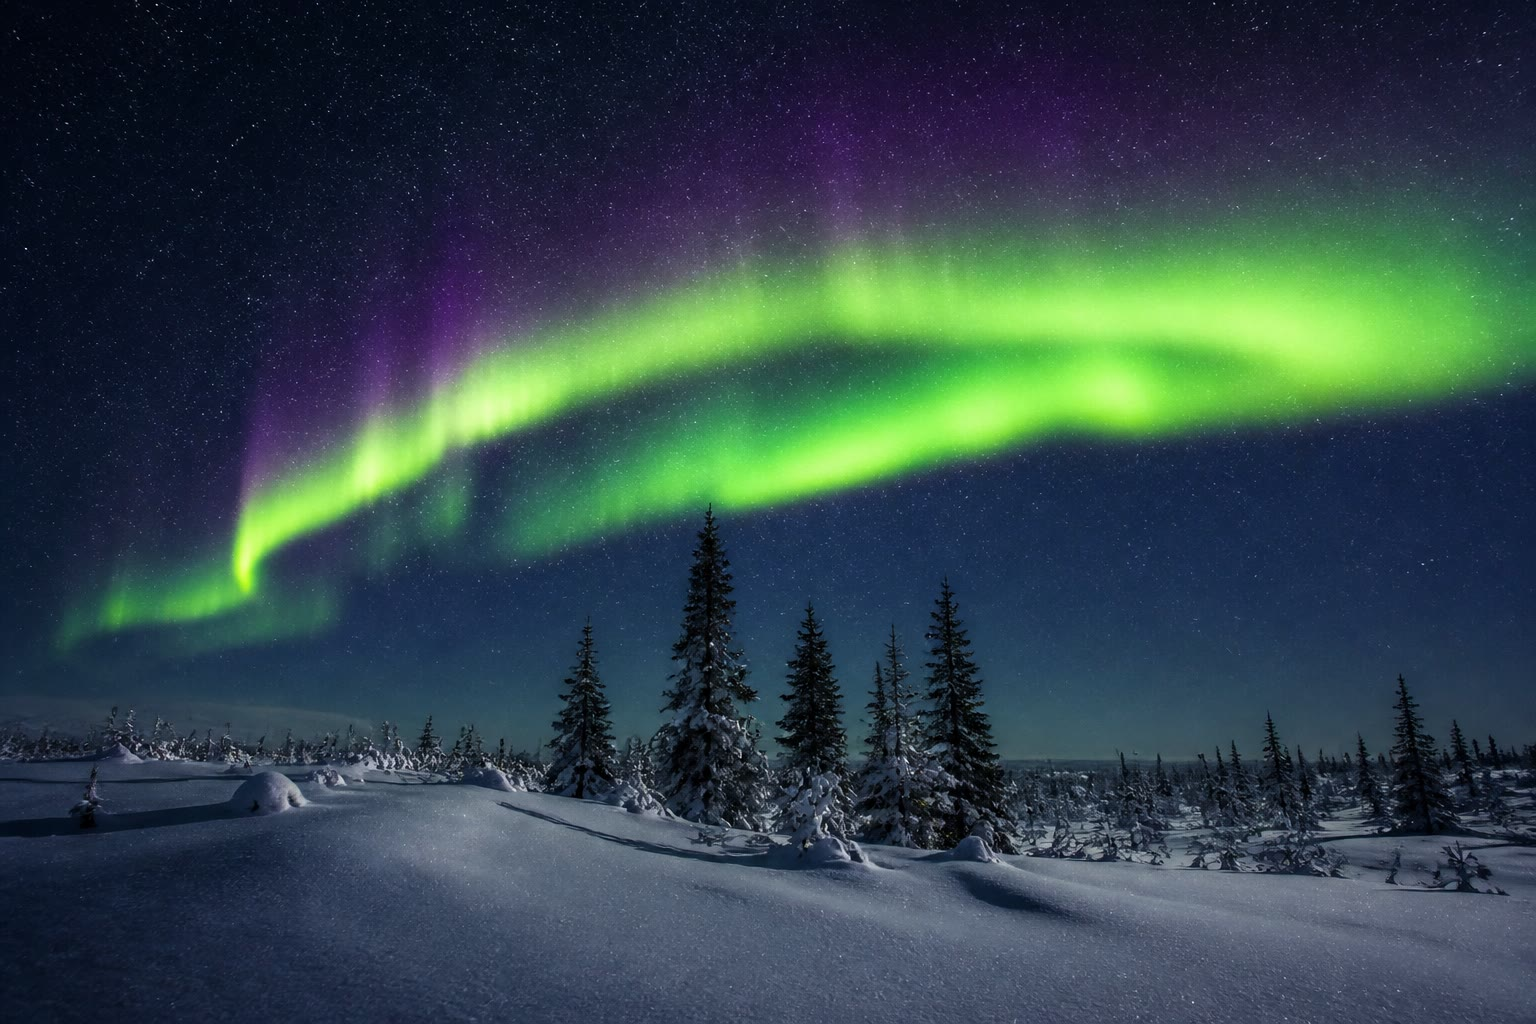
\includegraphics[width=0.58\linewidth]{images/book5/ai/b5-24-aurora-arc.jpg}

{\small Een poollicht: ladingen uit de zonnewind, door het magneetveld van de aarde de poolatmosfeer in gestuurd. Wat de ene waarnemer magnetische sturing noemt, noemt de andere elektrische versnelling --- de velden mengen onder de transformaties van dit hoofdstuk.}
\end{omfigure}

\section{Opgaven}

\begin{exercise}[$\star$]\label{exo:b3:covariant-electromagnetism:1}
(a) Boost $a^\mu = (5, 3, 0, 0)$ (in eenheden van een of andere $a_0$)
met $\beta =
0.6$: bereken $a'^\mu$ en ga na dat $a\cdot a$ onveranderd
blijft. (b) Toon aan dat de som van twee \omterm{def:b3:covariant-electromagnetism:fourvector}{viervectoren} een \omterm{def:b3:covariant-electromagnetism:fourvector}{viervector} is.
(c) Is $(c,
\vect v)$ van een deeltje een \omterm{def:b3:covariant-electromagnetism:fourvector}{viervector}? En $\gamma(c, \vect v)$? (d) Waarom maakt ``het elektrische veld'' alleen geen deel uit van
enige \omterm{def:b3:covariant-electromagnetism:fourvector}{viervector}?
\end{exercise}

\begin{exercise}[$\star$]\label{exo:b3:covariant-electromagnetism:2}
Een koperdraad met doorsnede \qty{1.0}{mm^2} voert \qty{10}{A}; de
dichtheid van de geleidingselektronen is $n = \qty{8.5e28}{m^{-3}}$. (a)
Bereken de driftsnelheid. (b) Schrijf $J^\mu$ op voor de
elektronenvloeistof en voor het rooster. (c) Ga voor elk de
continuïteitsvergelijking na. (d) De draad is neutraal: wat is $J^\mu$
voor de hele draad, en welke component overleeft?
\end{exercise}

\begin{exercise}[$\star$]\label{exo:b3:covariant-electromagnetism:3}
(a) Lees uit de matrix van $F^{\mu\nu}$ af welke componenten $E_y$ en
$B_x$ geven. (b) Schrijf $F^{\mu\nu}$ op voor een zuiver uniform veld
$\vect B = B\vect e_z$, en voor het veld van een vlakke golf ($\vect E = E\vect e_y$, $\vect B = (E/c)\vect e_z$). (c) Ga op de componenten na dat
$F^{\mu\nu} = \partial^\mu A^\nu - \partial^\nu
A^\mu$ de betrekking
$\vect B = \operatorname{\vect{curl}}\vect A$ oplevert voor $\mu\nu = 12$. (d)
Waarom moet $F$ antisymmetrisch zijn opdat de kracht $qF^{\mu\nu}u_\nu$
in het eigen stelsel van het deeltje geen arbeid verricht?
\end{exercise}

\begin{exercise}[$\star$]\label{exo:b3:covariant-electromagnetism:4}
Een vlakkeplaatcondensator in rust houdt $\vect E = E_0\vect e_y$ vast,
zonder $\vect B$. Geef $\vect E'$ en $\vect B'$ in een stelsel dat
beweegt (a) langs $\vect e_y$ (loodrecht op de platen); (b) langs $\vect
e_x$ (evenwijdig aan de platen), en duid de $\vect B'$ die verschijnt als
het veld van de bewegende oppervlakteladingen; (c) toets de invarianten in
geval (b); (d) in geval (b) krimpen ook de platen: welke grootheden
($\sigma$? $E'$? de plaatafstand?) veranderen, en in overeenstemming
waarmee?
\end{exercise}

\begin{exercise}[$\star\star$]\label{exo:b3:covariant-electromagnetism:5}
De bewegingsspanning verenigd. Een geleidende staaf glijdt met $\vect v$
over rails door een uniforme $\vect B$. (a) Boekhouding in het lab: welke
kracht drijft de elektronen langs de staaf, en welke spanning volgt
daaruit? (b) Boekhouding in het stelsel van de staaf: welk veld drijft ze,
en waar komt het vandaan in
\cref{prop:b3:covariant-electromagnetism:transform}? (c) Toon aan dat de
twee spanningen tot op de orde $v/c$ overeenstemmen. (d) De fluxregel van
Faraday uit het volume van jaar 1 dekte de gevallen ``bewegende kring'' en
``veranderend veld'' met één formule: wat zegt de relativiteitstheorie
over waarom die eenmaking wel moest werken?
\end{exercise}

\begin{exercise}[$\star\star$]\label{exo:b3:covariant-electromagnetism:6}
(a) Ga met \cref{prop:b3:covariant-electromagnetism:transform} door
rechtstreeks rekenen na dat $E'^2 - c^2B'^2 = E^2 - c^2B^2$ voor een boost
langs $x$. (b) Ga $\vect E'\cdot\vect B' = \vect
E\cdot\vect B$ na. (c)
Een gebied bevat loodrecht op elkaar staande $\vect E$ en $\vect B$ met
$E = 2cB$: bepaal het stelsel met een zuiver elektrisch veld (richting en
snelheid). (d) Waarom kan geen enkel stelsel het veld van een vlakke
lichtgolf zuiver elektrisch of zuiver magnetisch maken?
\end{exercise}

\begin{exercise}[$\star\star$]\label{exo:b3:covariant-electromagnetism:7}
Gekruiste velden. In het lab is $\vect E = E\vect e_y$ en $\vect B =
B\vect e_z$ met $E < cB$. (a) Toon aan dat het stelsel dat met $\vect v_{\text{d}} = (E/B)\,\vect e_x$ beweegt een zuiver magnetisch veld ziet.
(b) Beschrijf de beweging van een lading die uit rust wordt losgelaten,
gezien vanuit dat stelsel en weer terug in het lab (een cycloïde die met
$v_{\text{d}}$ meedrijft). (c) Het snelheidsfilter van het volume van jaar
1 liet deeltjes met snelheid $E/B$ onafgebogen door: leid dat in één regel
opnieuw af uit (a). (d) Wat gebeurt er kwalitatief wanneer $E > cB$ ---
en waarom is de truc met het driftstelsel dan onmogelijk?
\end{exercise}

\begin{exercise}[$\star\star$]\label{exo:b3:covariant-electromagnetism:8}
De viergolfvector $k^\mu = (\omega/c, \vect k)$. (a) Toon aan dat de eis
dat de fase invariant is, $k^\mu$ dwingt als \omterm{def:b3:covariant-electromagnetism:fourvector}{viervector} te transformeren.
(b) Leid de longitudinale dopplerformule uit zijn tijdcomponent af. (c)
Leid de aberratieformule af. (d) Aberratie van sterrenlicht: de aarde
draait rond met \qty{29.8}{km/s}; over welke hoek zwenkt de schijnbare
stand van een ster in een jaar? (Bradley mat in 1728 $20.5''$ --- het
eerste rechtstreekse bewijs dat de aarde beweegt.)
\end{exercise}

\begin{exercise}[$\star\star$]\label{exo:b3:covariant-electromagnetism:9}
Een lading $q$ beweegt met constante $\vect v = v\vect e_x$, $\gamma \gg
1$. (a) Toon door het veld van Coulomb te transformeren aan dat in het
dwarsvlak door de lading het veld tot $\gamma
q/4\pi\varepsilon_0b^2$ op
afstand $b$ wordt opgevoerd, terwijl het pal vooruit en achteruit met
$1/\gamma^2$ wordt platgedrukt. (b) Toon aan dat een stilstaande
waarnemer op afstand $b$ een veldpuls van duur $\sim b/\gamma v$ ziet. (c)
Voor een LHC-proton dat op $b = \qty{1}{cm}$ passeert: piekveld en
pulsduur. (d) In welke precieze zin is deze puls ``bijna licht''? (Ga $E' \approx cB'$ en de invarianten na.)
\end{exercise}

\begin{exercise}[$\star\star\star$]\label{exo:b3:covariant-electromagnetism:10}
Een lichtgolf achtervolgen. Een vlakke golf heeft $\vect E = E_0\vect e_y
\cos(\omega(t - x/c))$, $\vect B = (E_0/c)\vect e_z\cos(\omega(t -
x/c))$. Een waarnemer achtervolgt haar met $\beta$. (a) Transformeer de
velden: toon aan dat $E'_0 = E_0\sqrt{(1-\beta)/(1+\beta)}$ en $B'_0 = E'_0/c$. (b) Toon aan dat de frequentie met dezelfde factor transformeert:
de golf blijft een golf, roodverschoven, met altijd $E' = cB'$. (c) Wat
wordt er van de energiedichtheid van de golf (evenredig met $E^2$) en van
het aantal fotonen? (d) Concludeer: wat zou ``naast een lichtbundel
meerijden'' vergen, en welke invariant verbiedt het?
\end{exercise}

\begin{exercise}[$\star\star\star$]\label{exo:b3:covariant-electromagnetism:11}
Synchrotronlicht en de dood van de cirkelvormige elektronmachines. Een
ultrarelativistische lading op een cirkel met straal $r$ straalt het
vermogen $P = q^2c\gamma^4/6\pi\varepsilon_0r^2$ uit (aangenomen --- de
formule van Larmor uit het volume van jaar 2, geboost). (a) Toon aan dat
het energieverlies per omloop $\Delta E = q^2\gamma^4/3\varepsilon_0r$
bedraagt. (b) LEP: elektronen van \qty{100}{GeV} op $r = \qty{3.1}{km}$:
bereken $\gamma$ en $\Delta E$ per omloop --- welk deel van de
bundelenergie wordt elk rondje teruggekocht? (c) LHC: protonen van
\qty{6.8}{TeV} in dezelfde tunnel: bereken $\Delta E$ per omloop en
vergelijk. (d) Verklaar met de factor $\gamma^4 =
(E/mc^2)^4$ waarom de
opvolger van de elektronen een \emph{lineaire} botser of een veel grotere
ring is, en waarom protonringen wel overleven.
\end{exercise}

\begin{exercise}[$\star\star\star$]\label{exo:b3:covariant-electromagnetism:12}
Het relativistische cyclotron. Een lading in een uniforme $\vect B$, bij
relativistische snelheid. (a) Toon uit $\dd\vect p/\dd t = q\vect v\wedge\vect
B$ met constante $E$ aan dat de baan een cirkel is die met $\omega = qB/\gamma m$ wordt doorlopen: de cyclotronfrequentie daalt met de energie.
(b) Een klassiek cyclotron duwt met vaste $\omega_0 = qB/m$: toon aan dat
na $N$ omlopen, waarbij $\gamma - 1$ lineair tot zijn eindwaarde $\Gamma$
groeit, de opgehoopte faseachterstand een kwart RF-periode bereikt zodra
$\Gamma \approx 1/2N$; welke kinetische energie van een proton is dat voor
$N = 100$ omlopen, en hoe verhoudt zij zich tot het historische plafond
van klassieke cyclotrons (zo'n \qty{20}{MeV}, gekocht met extra marge en
spanning)? (c) Er bestaan twee remedies: de frequentie laten meelopen
(synchrocyclotron) of $B(r)$ zo vormen dat het als $\gamma$ groeit
(isochroon cyclotron): leg elk in één zin uit. (d) Het isochrone cyclotron
van het PSI levert protonen van \qty{590}{MeV}: met welke factor
overtreft zijn veld aan de rand het veld in het midden?
\end{exercise}

\section{Vraagstuk: Magnetisme op slakkengang}

\begin{problem}[{Weekendvraagstuk --- hoe een onevenwicht van $10^{-24}$
elke motor laat draaien}]\label{pb:b3:covariant-electromagnetism:1}
Elektronen driften trager door een lampsnoer dan honing kruipt, en
$v^2/c^2$ voor die drift is $10^{-24}$ --- en toch tilt de magnetische
kracht die zij voortbrengt auto's op sloopterreinen. Dit vraagstuk maakt
de volledige boekhouding in twee stelsels op voor een rechte draad en een
bewegende lading, en vindt de relativiteitstheorie in elke elektromagneet
terug. Gegevens: koperdraad, doorsnede $S = \qty{1.0}{mm^2}$, stroom $I = \qty{10}{A}$, dichtheid van de geleidingselektronen $n = \qty{8.5e28}{m^{-3}}$; proeflading $q = \qty{1}{\micro C}$ op afstand $d = \qty{1.0}{cm}$, die evenwijdig aan de draad met $v = \qty{e5}{m/s}$
beweegt (de snelheid van een ionenbundel, om de getallen zichtbaar te
houden); $\mu_0 = 4\pi\times10^{-7}\,\unit{H/m}$.

\medskip\noindent\textbf{Deel I --- De boekhouding in het lab.}
\begin{enumerate}
  \item Bereken de driftsnelheid $u$ van de elektronen, en $u^2/c^2$.
  \item Modelleer de draad als twee over elkaar heen liggende
        lijnladingen: het rooster $+\lambda$ in rust en de elektronen
        $-\lambda$ driftend met $u$, met $I = \lambda u$. Bereken
        $\lambda$.
  \item Bereken $B$ op de plaats van de lading en de magnetische kracht
        $F = qvB$ erop --- inclusief richting, voor een $v$ evenwijdig
        aan de conventionele stroom $I$ (denk eraan: evenwijdige stromen
        trekken elkaar aan).
  \item Waarom is er in het lab geen \emph{elektrische} kracht?
  \item Het elektrische veld van dezelfde draad als die per meter een
        netto overschot van één elektron droeg: vergelijk de kracht die
        dat op $q$ zou uitoefenen met de magnetische kracht uit vraag 3,
        en concludeer hoe nauwkeurig ``neutraal'' moet worden gemeten
        voordat men iets aan magnetisme mag toeschrijven.
  \item Een lading van \qty{1}{\micro C} met \qty{e5}{m/s}: is de kracht
        uit vraag 3 meetbaar? (Vergelijk met het gewicht van een
        zandkorrel, $\sim\qty{e-6}{N}$.)
\end{enumerate}

\medskip\noindent\textbf{Deel II --- Van stoel wisselen.}
Boost naar het stelsel van de proeflading (snelheid $v$ langs de draad).
\begin{enumerate}[resume]
  \item Welke snelheden hebben in dat stelsel het rooster en de
        elektronen (die tegen $I$ in driften en in deze boost dus
        sneller worden --- stel ze netjes samen)?
  \item Over de doorsnede van de draad geïntegreerd is de vierstroom per
        eenheid van lengte $(c\lambda_{\text{tot}}, I, 0, 0)$, hier met
        $\lambda_{\text{tot}} = 0$. Transformeer haar en toon aan dat de
        lijnlading van de draad in het nieuwe stelsel
        \[
        \lambda' = -\gamma_v\,\frac{vI}{c^2} .
        \]
  \item Bereken $\lambda'$, in coulomb per meter en in
        elektronladingen per meter. Welke stroom werd dichter, en
        waarom (krimp desgewenst elke stroom afzonderlijk)?
  \item Bereken het elektrische veld $E' = \lambda'/2\pi\varepsilon_0d$
        op de lading, en de elektrische kracht $qE'$ erop.
  \item Vergelijk $qE'$ met de $qvB$ van het lab uit deel I, en verklaar
        de resterende factor $\gamma_v \approx 1 + \num{5.6e-8}$ (de
        transformatiewet van welke \omterm{def:b3:covariant-electromagnetism:fourvector}{viervector} verbindt de krachten?).
  \item In dit stelsel is er ook een magnetisch veld (de draad voert nog
        steeds stroom): waarom oefent dat hier geen kracht uit?
\end{enumerate}

\medskip\noindent\textbf{Deel III --- De moraal van de getallen.}
\begin{enumerate}[resume]
  \item Het relatieve onevenwicht $|\lambda'|/\lambda$: bereken het en
        schrijf het als $\gamma_v vu/c^2$.
  \item Hoe kan een effect van de orde $10^{-19}$ van de lading van de
        draad een macroscopische kracht opleveren? (Welk enorm getal
        vermenigvuldigt het?)
  \item Twee evenwijdige draden met elk \qty{10}{A} op \qty{1}{cm}:
        bereken de kracht per meter en toets haar aan de
        definitiewaarde $2 \times 10^{-7}\,I_1I_2/d$ newton per meter.
  \item Een elektromagneet is tienduizend windingen van dit verhaal:
        schat het veld van een spoel met \qty{e4}{} windingen per meter
        die \qty{10}{A} voert (de solenoïdeformule van het volume van
        jaar 1), en de kracht per vierkante centimeter die zij op ijzer
        uitoefent ($\sim B^2/2\mu_0$).
  \item Zou de relativiteitstheorie worden uitgeschakeld ($c \to \infty$
        in de transformatie), wat bleef er dan over van $\lambda'$, van
        de kracht van $B$, van motoren en sloopmagneten?
  \item Waarom voelt de proeflading die \emph{in rust} bij de draad ligt
        niets, hoewel de elektronen langs haar stromen? (Welke
        opheffing beschermt haar, en tot op welke nauwkeurigheid?)
\end{enumerate}

\medskip\noindent\textbf{Deel IV --- Voorbij de draad.}
\begin{enumerate}[resume]
  \item Het volume van jaar 2 leidde magneetvelden af uit de wet van
        Ampère met stromen als gegeven bronnen. Wat voegt dit
        hoofdstuk daaraan toe --- wat \emph{is} het magneetveld, gezien
        vanuit dit vraagstuk?
  \item IJzeren magneten hebben geen batterij: wat speelt bij permanent
        magnetisme de rol van de stroom (één zin; het eerlijke
        microscopische antwoord is kwantummechanisch en wacht vijf
        hoofdstukken)?
  \item Eén enkele elektronenbundel in vacuüm (zonder rooster): ziet een
        meebewegende waarnemer haar zichzelf sterker aantrekken of
        afstoten dan een waarnemer in het lab? Verzoen de boekhouding
        van de twee stelsels over het samenknijpen van een bundel.
  \item Maak dat laatste punt kwantitatief: toon aan dat twee
        evenwijdige gelijkgeladen bundels die samen met $\beta$ bewegen
        elkaar afstoten met een netto kracht (elektrische afstoting min
        magnetische aantrekking) die precies met $1/\gamma^2$ onder haar
        rustwaarde ligt --- en zeg in welk stelsel die factor
        vanzelfsprekend is.
  \item De energie voor een lamp komt met bijna $c$ aan, terwijl haar
        elektronen een meter per uur driften: wat draagt de energie in
        werkelijkheid langs het snoer (denk aan de poyntingvector van
        het volume van jaar 2)?
  \item Schat $vu/c^2$ voor de elektronen van dit vraagstuk en een
        proeflading op wandeltempo ($v = \qty{1}{m/s}$): zelfs daar is
        de kracht in eerste orde meetbaar met een kompasnaald --- wie
        toonde aan dat stroom een kompas afbuigt, en in welk jaar?
  \item Vat het genoemde resultaat samen: een neutrale draad van
        \qty{10}{A}, bekeken vanaf een stoel die met \qty{e5}{m/s}
        beweegt, draagt $-\qty{e-11}{C/m}$ aan relativistische lading
        --- en die boekhoudfout van de orde $10^{-24}$ door \omterm{prop:b3:relativistic-kinematics:contraction}{lengtekrimp},
        vermenigvuldigd met $10^{28}$ elektronen, is de volledige
        magnetische kracht van het lab.
\end{enumerate}
\end{problem}
